\Section*{Galerkin approach}

\begin{frame}{Continuous Galerkin (CG) method\myfootcite{Ern2004}}
	\begin{minipage}[t]{0.62\linewidth}
		For a \coloredonly<1>{fixed $\bm{\mu}\in\mathcal{M}$}, let $\mathcal{T}_h$ be a mesh of $\Omega$.

		\vspace{5pt}

		Let $V_h$ be a \coloredonly<1>{continuous space} of piecewise polynomials of degree $k$ on $\mathcal{T}_h$. Its basis functions $(\phi_i)_i$, with $\phi_i$ supported on the cells sharing the dof $i$, decompose the discrete solution:
		\vspace{-8pt}
		\[
			u_h(\bm{x},\bm{\mu}) = \sum_{i=1}^{N_\text{dofs}}\beta_i(\bm{\mu})\,\phi_i(\bm{x}).
		\]
	\end{minipage} \hfill \begin{minipage}[t]{0.36\linewidth}
		\vspace{-20pt}
		\centering
		\includegraphics[page=2]{images/background/cg_basis/cg_basis.pdf}
	\end{minipage}

	\vspace{3pt}
	\blk{2}{%
		\textbf{Variational problem:} \quad Find $u_h\in V_h^0$ such that, $\forall v_h\in V_h^0$, $a(u_h,v_h;\bm{\mu})=l(v_h;\bm{\mu})=\int_\Omega f\,v_h$,

		\vspace{-3pt}
		\begin{equation*}
			a(u_h,v_h;\bm{\mu}) = \int_\Omega \Big(R\, u_h v_h + \bm{C}\cdot\nabla u_h\, v_h + \frac{1}{\text{Pe}} D\nabla u_h\cdot\nabla v_h\Big)
		\end{equation*}
		\vspace{-10pt}

		with $V_h^0\subset V_h$ \coloredonly<2>{vanishing on $\Gamma$} (homogeneous Dirichlet condition).
	}

	\vspace{3pt}
	\blk*{3}{%
		\textbf{Linear system:}
		\vspace{-3pt}
		\[
			\underset{\text{\footnotesize matrix}}{A_h(\bm{\mu})}\;\underset{\text{\footnotesize dofs}}{\bm{\beta}_h(\bm{\mu})}=\underset{\text{\footnotesize right-hand side}}{\bm{b}_h(\bm{\mu})},
			\qquad A_{ij}=\coloredonly<3>{a(\phi_j,\phi_i;\bm{\mu})},\quad b_i=\coloredonly<3>{l(\phi_i;\bm{\mu})}
		\]
	}
\end{frame}


% tableau de la slide « Link between Galerkin and PINNs » : colonne étroite à gauche pour la pastille d'étape (\multirow centrée sur le bloc de lignes)
\newenvironment{cmptabn}{\begin{tabular}{@{}>{\centering\arraybackslash}p{0.03\linewidth}@{\hspace{5pt}}p{0.16\linewidth}>{\centering\arraybackslash}p{0.36\linewidth}>{\centering\arraybackslash}p{0.38\linewidth}@{}}}{\end{tabular}}

\Section*{Learning-based approaches}

\begin{frame}{Physics-informed neural networks (PINNs)\myfootcite{Raissi2019}}
	Let $u_\theta(\bm{x},\bm{\mu})$ be a \coloredonly<1>{neural network} with weights $\theta$ and inputs $(\bm{x},\bm{\mu})\in\Omega\times\mathcal{M}$, approximating the solution $u$.

	\vspace{7pt}
	\textbf{Training:} \quad Find the weights $\theta^\star$ such that
	\vspace{-3pt}
	\begin{equation*}
		\theta^\star = \argmin_\theta \big( \omega_r\,\mathcal{J}_r(\theta) + \omega_b\,\mathcal{J}_b(\theta) \big) \tag{$\mathcal{P}_\theta$},
	\end{equation*}
	with $\omega_r$ and $\omega_b$ the weights of the two loss terms, and

	\vspace{6pt}
	\begin{minipage}{0.8\linewidth}
		\begin{equation*}
			\begin{aligned}
				\text{\textcolor{darkred}{\footnotesize residual loss}} \;\; & \fcolorbox{darkred}{white}{$\displaystyle \mathcal{J}_r(\theta) = \int_{\mathcal{M}}\int_\Omega \big|\mathcal{L}\big(u_\theta(\bm{x},\bm{\mu});\bm{x},\bm{\mu}\big)-f(\bm{x},\bm{\mu})\big|^2\,\mathrm{d}\bm{x}\,\mathrm{d}\bm{\mu}$,} \\[4pt]
				\text{\textcolor{orange}{\footnotesize boundary loss}} \;\;  & \fcolorbox{orange}{white}{$\displaystyle \mathcal{J}_b(\theta) = \int_{\mathcal{M}}\int_\Gamma \big|u_\theta(\bm{x},\bm{\mu})\big|^2\,\mathrm{d}\bm{x}\,\mathrm{d}\bm{\mu}$.}
			\end{aligned}
		\end{equation*}
	\end{minipage}

	\vspace{7pt}
	\textbf{Monte-Carlo method:}

	Discretize the cost functions by random process.

	% réseau en bas à droite, hors flux du texte (ne décale rien) ; visible sur tous les overlays
	\begin{tikzpicture}[remember picture,overlay]
		\node[anchor=south east,inner sep=0pt] at ([xshift=-0.5cm,yshift=0.75cm]current page.south east) {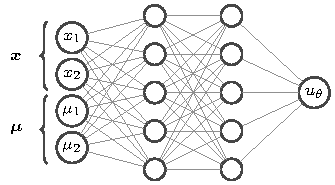
\includegraphics[width=5cm]{images/background/network/network.pdf}};
	\end{tikzpicture}
\end{frame}

\Section*{Common framework}

\begin{frame}{Link between Galerkin and PINNs}
	\renewcommand{\arraystretch}{1.15}
	\textbf{Numerical method (three steps):} \hfill \only<4>{\coloredonly<4>{\textbf{Same philosophy, different approximation space}}}

	\vspace{-8pt}
	\centering
	\only<1>{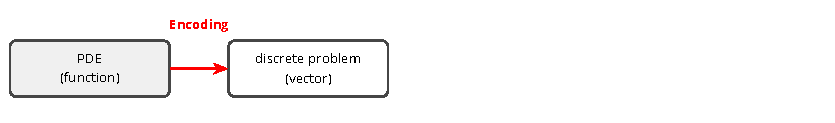
\includegraphics[page=1]{images/background/encdec/encdec.pdf}}%
	\only<2>{\includegraphics[page=2]{images/background/encdec/encdec.pdf}}%
	\only<3>{\includegraphics[page=3]{images/background/encdec/encdec.pdf}}%
	\only<4->{\includegraphics[page=4]{images/background/encdec/encdec.pdf}}

	\vspace{4pt}
	\begin{cmptabn}
		\toprule
		& & \textbf{Galerkin (CG)}                     & \textbf{PINN}                                       \\
		\midrule
		\multirow{3}{*}{\stepcirc{1}} & Space                      & vector space $V_h$                    & manifold of the $u_\theta$                          \\
		& Unknowns                   & dofs $\bm{\beta}_h(\bm{\mu})$           & weights $\theta$                                    \\
		& Integrals                  & quadrature on cells                   & Monte Carlo on collocation points                   \\
	\end{cmptabn}%

	\only<2->{%
		\begin{cmptabn}
			\midrule
			\multirow{2}{*}{\stepcirc{2}} & Parameters                  & \leavevmode\coloredonly<2>{fixed $\bm{\mu}$}, one solve per $\bm{\mu}$ & \leavevmode\coloredonly<2>{$\bm{\mu}\in\mathcal{M}$ as input}, one training \\
			& Resolution                  & linear system $A_h(\bm{\mu})\bm{\beta}_h(\bm{\mu})=\bm{b}_h(\bm{\mu})$ & optimization on $\theta$                        \\
		\end{cmptabn}%
	}

	\only<3->{%
		\begin{cmptabn}
			\midrule
			\stepcirc{3} & Solution                    & $u_h(\bm{x},\bm{\mu})$, \coloredonly<3>{linear} in $\bm{\beta}_h$ & $u_\theta(\bm{x},\bm{\mu})$, \coloredonly<3>{non-linear} in $\theta$ \\
			\bottomrule
		\end{cmptabn}%
	}
\end{frame}
